\documentclass{report}
\usepackage{graphicx}
\usepackage[round]{natbib}
%\usepackage[backend=biber]{biblatex}
%\addbibresource{bib.bib} % with extension


\begin{document}

\author{Hamid Shayestehmanesh}
\title{Creating a instrument based on movements in webcam view}
\maketitle
\tableofcontents
\newpage

\section{Main Project Idea}

The main problem this project is based is to build a HCI application which can shape the music. In other words, we want to design and build an application which is able to translate hands movements to meaningful sounds and build a new electronic music instrument.
\subsection{More Specified}
In this project we are following the goal to design an architecture of such program and building a prototype. To detect hands movement we use different colored cameras and regular speakers to generate sounds. Devices and implementation environment will be discussed in details later.
\pagebreak


\section{Literature}
This section is the most important section in the report. All next parts are based on information explained in this chapter. This section tries to translate needed knowledge of music from musician language to computer scientists language. 
\subsection{Music Language and Important Information}
any one of the systems of signs and words that are used by a particular group of people to communicate and transfer knowledge about a specific subject is called a language\citep{Lang}. Nowadays, translation has become very common but, it faces different difficulties. Finding the best word in destination language, demonstrating emotions and feelings and, keeping the structure of the article are some of the hardest problems of translating. Here, we are trying to translate language of a musician to an engineer language. So, we will explain different important aspect of musical notes which are mandatory to know about while building a new instrument.  

time
frequency
fasele hashoon, 
beka
oun yeki ke be bala miraft
just this!
anything else Sara ?
\subsubsection{Conclusion}
time 
frequency


\subsection{Important Information that are not in note Language}
an example of difference
power of the note
nesbateshoon
beat
any other information that a conductor may change!

\subsection{More Information about music}
parde ha




\pagebreak
\section{First Sample}
To decide what can be build practically we should have a minimal model of the system first.

\subsection{Abstract}
A minimal model implemented using Python, OpenCV(Tracking the Object) and Pygame(Generating Sounds). In this model moving the element (conductor baton) Vertically changes the frequency of sound and moving it horizontally changes sounds' amplitude. Coordination of the element identified by color segmentation. \newline Movement of the element also was computed using it's coordination in previous frame.
\subsection{Details}
The sample code works with one specific element. The idea was to clean all the view of the webcam from one color and create that element in that color, so filtering on that color will let us to find the element easily. Filtering the color or color segmentation will give us a black and white frame which everything should be black but the element. In practice some other small areas will be converted to white, to solve this problem the image has to be cleaned. \textit{Eroding} and \textit{dilating} the image will fairly solve our problem here. In next step we should identify the element by one point to track it's movement,thus to do this first draw a contour around the white color. As the contour won't usually have a good shape, finding the minimum circle around the contour can give us a good presentation of the element coordination in frame, also center of circle is a good one-point identifier. \newline
Well now comparing two last center of this imaginary circle can help us detect any movement of the element. Now that the movement is detected, we can update our frequency and amplitude. Generate and play a sound with specified frequency and amplitude using Pygame. 

\section{Object Tracking}
The idea is to move and click with mouse using object movements in the read frame from camera. 
\subsection{Improving the Tracking system}
\subsubsection{Step 1}
The first two Objects are recognized by their size and color in the picture. The problem with these two objects is that if any object with the same color appears in the frame and has an appropriate size, the system will follow the wrong object of it will repeatedly change the recognized object between the correct one and the other, so the system is not robust. \newline
\begin{center}
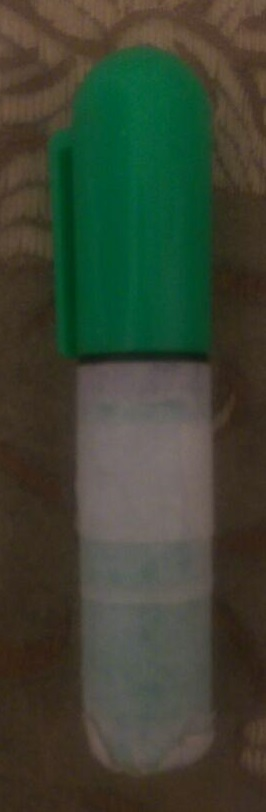
\includegraphics[width=1in]{Object1.jpg}
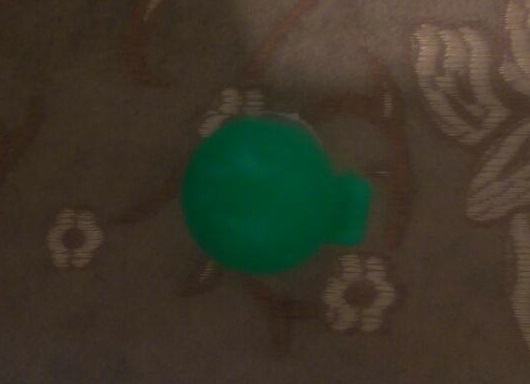
\includegraphics[width=3in]{Object1-2.jpg}\newline \figurename{Object1} Used from top (second image)	
\end{center}
\subsubsection{Step 2}
One easy idea to solve the problem is to increase the size of the object.
\begin{center}
	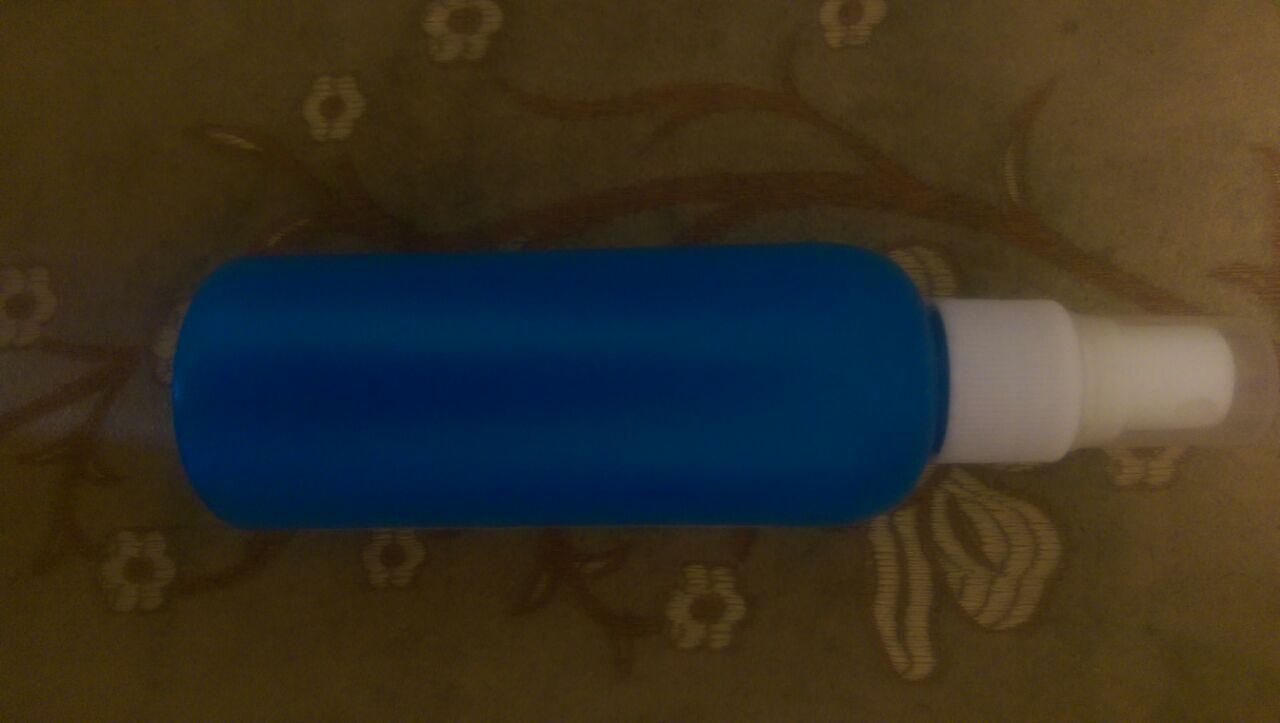
\includegraphics[width=3in]{Object2.jpg} \newline \figurename{Object2} Used from side 
\end{center}
Due to the fact that this step still recognize the object by size and color increasing the size won't help, mostly because of noises, sometimes the contour around the detected color becomes small specially in fast pace movements.  (Notice that system searches for a hard coded size of contour.)
\subsubsection{Step 3}
One Idea to solve the problem is to create a specific background, therefore the colored point won't be lost in the background color. First attempt with this idea is one stick on hand. \newline
\begin{center}
	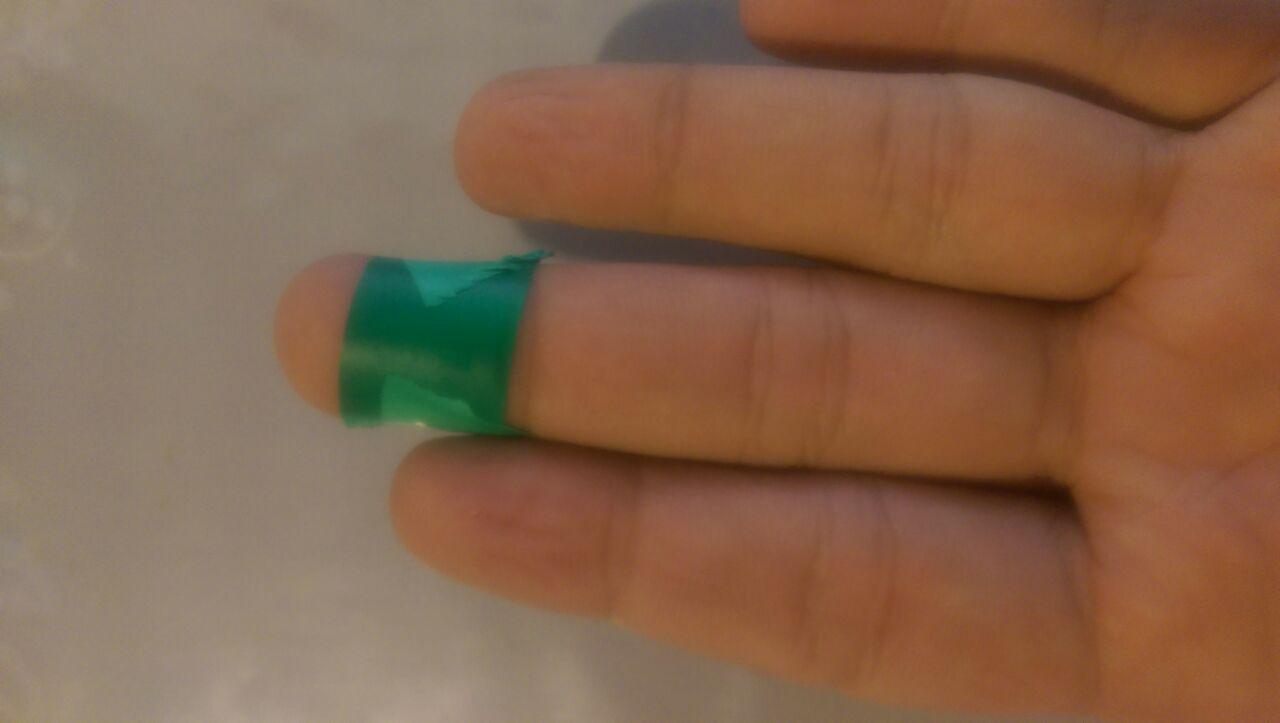
\includegraphics[width=3in]{Object3.jpg}\newline \figurename{The green color was seperated to detect the point}
\end{center}
\subsubsection{Step 4}
Even though a green stick on the finger seems detectable but in practice the color of skin is not very stable so it isn't very helpful as a background, also in light has a enormous effect on the color.
\subsubsection{Step 5}
To solve the problem some red stick are added in up and down and then on left and right. Even the system works fine with only  up and down red sticks but adding left and right ones will help the system when very bright lights exists in the frame.
\begin{center}
	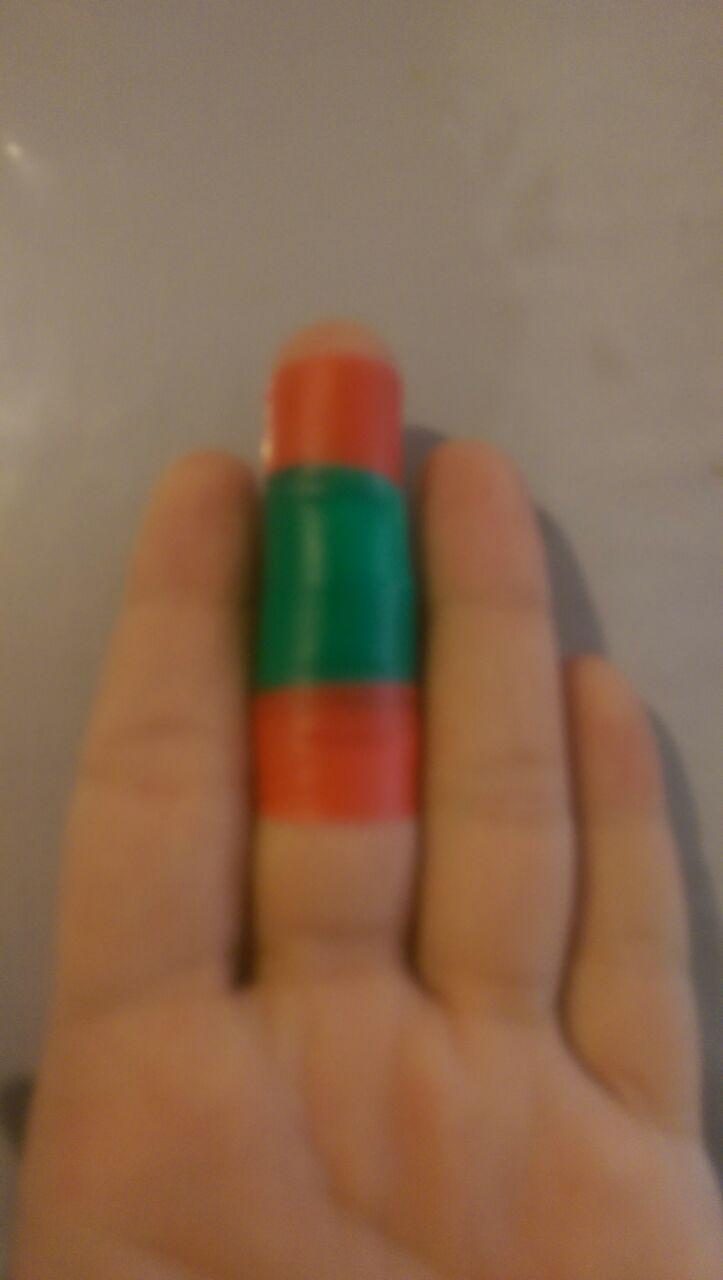
\includegraphics[width=2in]{Object4.jpg}
	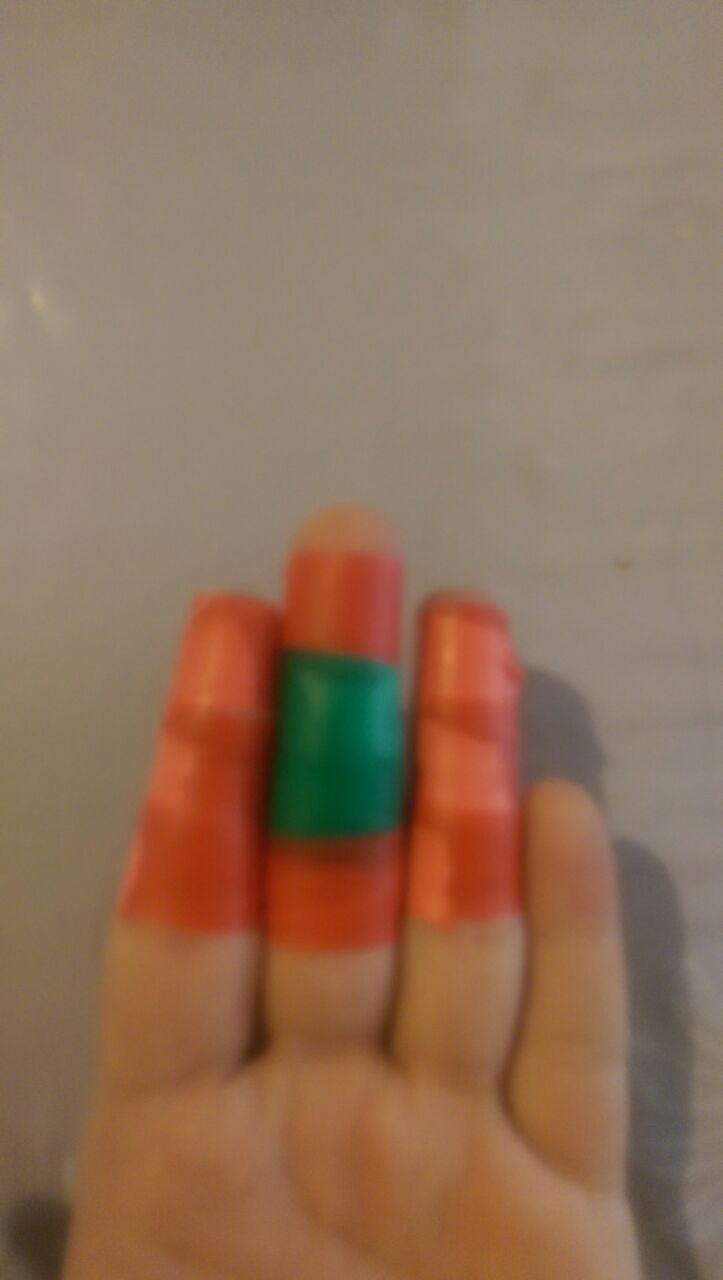
\includegraphics[width=2in]{Object5.jpg}
\end{center}
Due to the fact that sticks are very annoying I created something with papers.
\begin{center}
	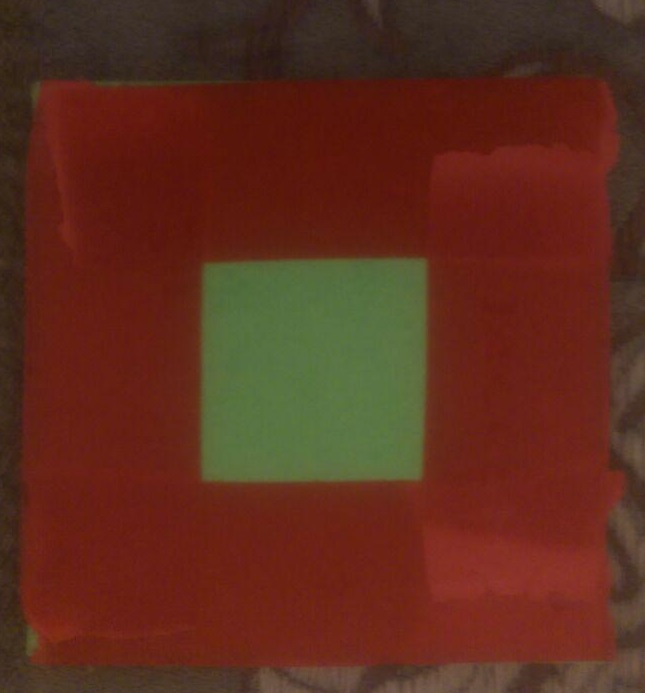
\includegraphics[width=2in]{Object6.jpg} \newline
	\figurename{Created with papers}
\end{center}

\subsubsection{Step 6}
The papered object worked fine but because of the small background sometimes following the point became hard. To solve the problem we use the fact that one's hand won't move very fast, so if call current position of point $p_1 = (x_1, y_1)$ and next position $p_2 = (x_2, y_2)$ then the distance between $p_1, p_2$ is less than $C$. So if we know the place of point, so we don't have to search the hole next frame to find the point. We have to search only a part of it, so a square with upper left point of $p_1 - (C, C)$ and the lower right point of $p_1 + (C, C)$ 
\subsubsection{Step 7}
If we could ever make the background bigger the system could work more robust. We created a glove with the point one it. The big background it used to create help the system to track the point using only mentioned square. 
\begin{center}
	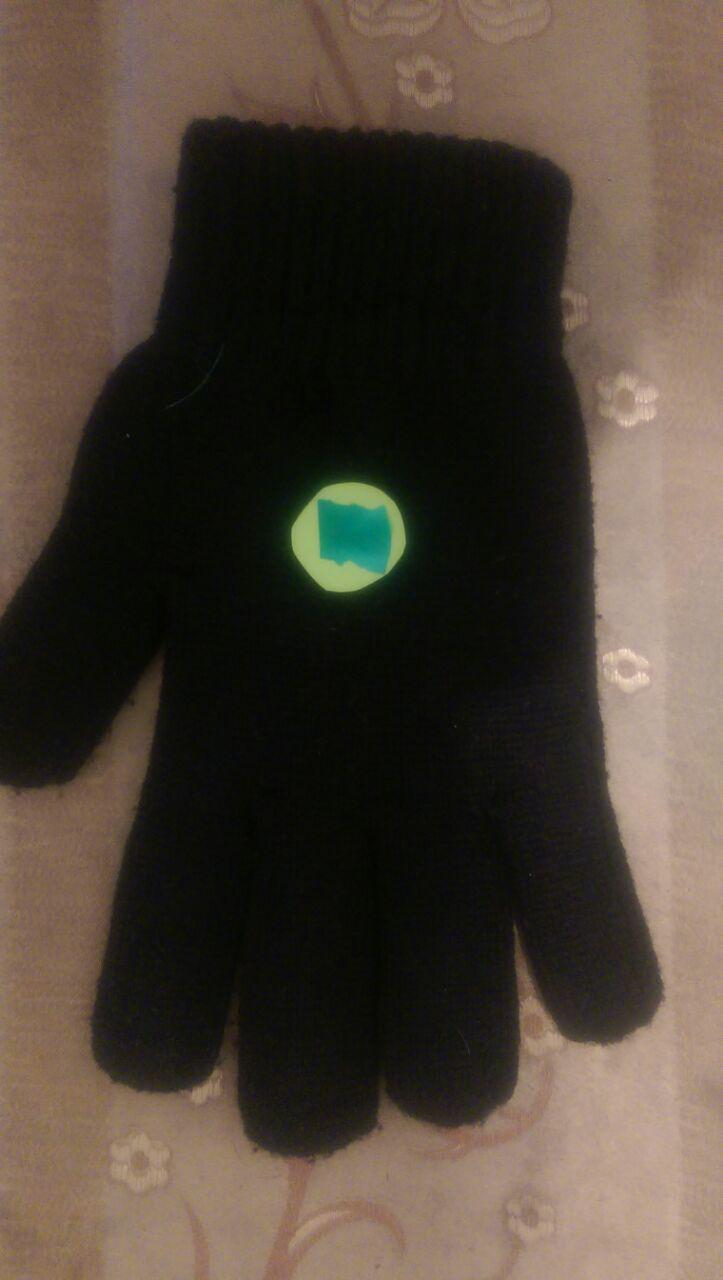
\includegraphics[width=3in]{Object7.jpg}
\end{center}
This object works very well but yet light can make huge distractions. To solve the problem we change many different color for the glove ( as the background ) (Colors are shown below) and the Red Dark seemed to work better than others. 
\begin{center}
	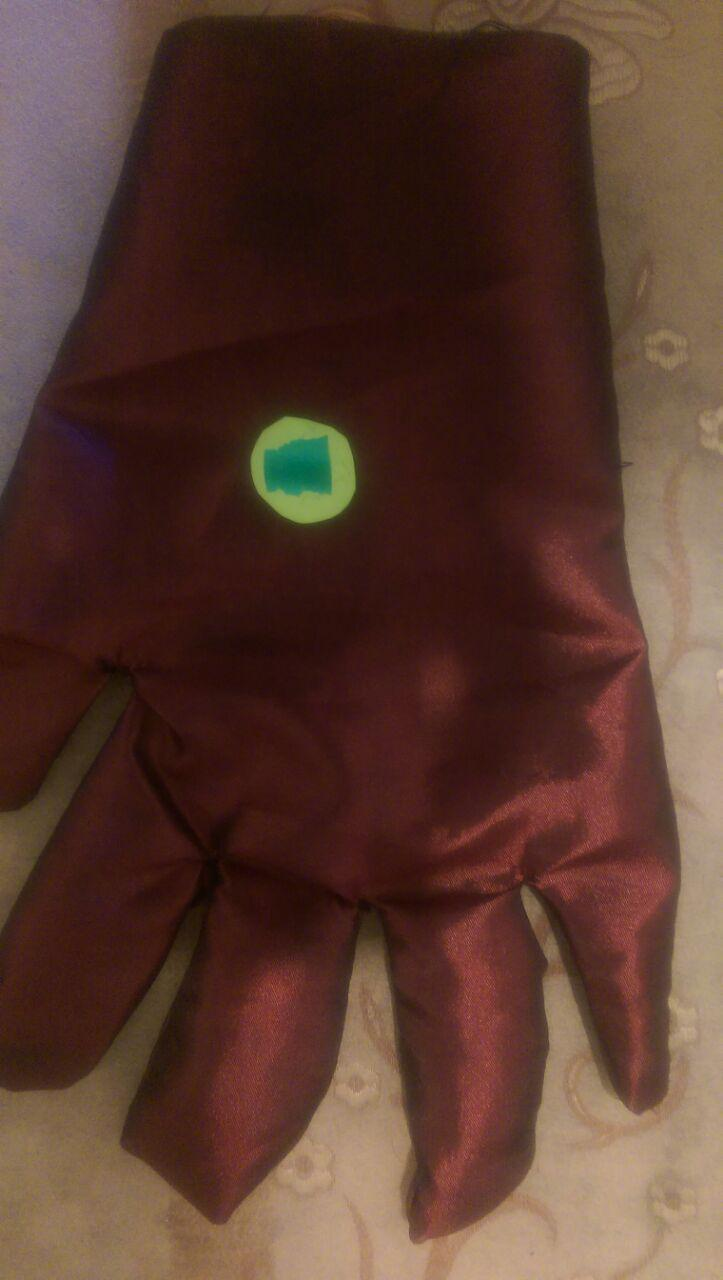
\includegraphics[width=3in]{Object8.jpg}
\end{center}

\section{Playing Notes}
To play notes we break the frame into 9 parts, one for silence and 8 others for 8 different notes. Shown below.


\section{Future Work}
It can be implemented on Android or any other mobile frameworks.
\section{Other Technologies}
A programming language called Chuck has been created in Princeton university. ChucK is a programming language for real-time sound synthesis and music creation. The problem with this language is that it's doesn't support any library which can use webcam or any type of camera, neither easy way to connect it to another programming language.
\bibliographystyle{plainnat}
\bibliography{bibfile}

\end{document}